% Created 2022-05-23 Mon 23:09
% Intended LaTeX compiler: pdflatex
\documentclass[11pt]{article}
\usepackage[utf8]{inputenc}
\usepackage[T1]{fontenc}
\usepackage{graphicx}
\usepackage{longtable}
\usepackage{wrapfig}
\usepackage{rotating}
\usepackage[normalem]{ulem}
\usepackage{amsmath}
\usepackage{amssymb}
\usepackage{capt-of}
\usepackage{hyperref}
\usepackage{cleveref}
\usepackage{subfig}
\usepackage[letterpaper, margin=1in]{geometry}
\usepackage{fancyhdr}
\pagestyle{fancy}
\fancyhead[CO,CE]{\textbf{[Align-BDD]}}
\fancyhead[LO,LE]{A.B.}
\fancyhead[RO,RE]{The Applications question.}
\author{Alexey Bochkarev}
\date{\today}
\title{On special classes of instances for align-BDD}
\hypersetup{
 pdfauthor={Alexey Bochkarev},
 pdftitle={On special classes of instances for align-BDD},
 pdfkeywords={},
 pdfsubject={},
 pdfcreator={Emacs 29.0.50 (Org mode 9.5.2)}, 
 pdflang={English}}
\begin{document}

\maketitle
In a nutshell:
\begin{itemize}
\item First, I looked into \emph{typed UFLP} on 'cavemen' graph structure and checked if
anything would change if the order of variables in the type diagram would be
randomized before alignment. It seems our heuristic does find smaller diagrams
more often than not. But for some reason this does not really yields benefit
in runtimes, as compared to a simple \texttt{align-to-A} heuristic.
\item Second, I tried to invent another problem, \emph{joint-UFLP}, and it seems this is where the
heuristic does make sense.
\end{itemize}

\textbf{My key question to you:} do you think the \emph{j-UFLP} would work / is it too
artificial?

\textbf{My next steps:} I'd need to double-check the experiment. Maybe there is a
cleaner way to generate a j-UFLP instance + add cross-checks here and there.
After that, if you think it is worth trying, I could set up a larger experiment
(increase the number of instances) and write everything up carefully + edit the
responses to the reviewers (in the \href{https://docs.google.com/document/d/1ArI6yFf6EnCjfm0r3Qogb1VRAa4eLkKdVQ-NB9QtuZQ/edit?usp=sharing}{google-doc} I sent before).


\section{UFLP with overlaps: general info}
\label{sec:org912bfcd}
We have been discussing variations of uncapacitated facility location problem
(UFLP). Let me try to lay out everything briefly, this way it seems easier to
spot problems in the logic. First, what we already had in the paper:
\begin{itemize}
\item We have an undirected graph, and I can \emph{locate a facility} at each point
(vertex), at cost \(c_i\) for the i-th point.
\item If a facility is located at point \(i\), it 'covers' all the points from its
neighborhood, \(S_i\) (which by convention includes \(i\)).
\end{itemize}

New things:
\begin{itemize}
\item \textbf{Overlap costs}. If a point \(j\) is covered \(a\) times, we bear cost (or profit)
\(f_{ja}\), with no particular assumptions on the structure of \(f_{ja}\)
depending on \(a\) (i.e., no monotonicity / convexity / concavity).
\item \textbf{Objective:} We do not demand all points to be covered, but we assume certain cost \(f_{j0}\)
for not covering a point at all. The objective is to minimize the sum of
costs, including location costs and overlap costs.
\item \textbf{Special structure / 'cavemen':} We restricted our attention to a special type
of instances, where points are split into clusters, with many edges within a
cluster, but only a single edge between two clusters (and each cluster being
connected to at most two other ones). An example of such instance is provided
in Fig. \ref{fig:ex-inst}. Note that I further refer to the endpoints of an edge
connecting two clusters as \emph{connection points}.
\end{itemize}

\begin{figure}[htbp]
\centering
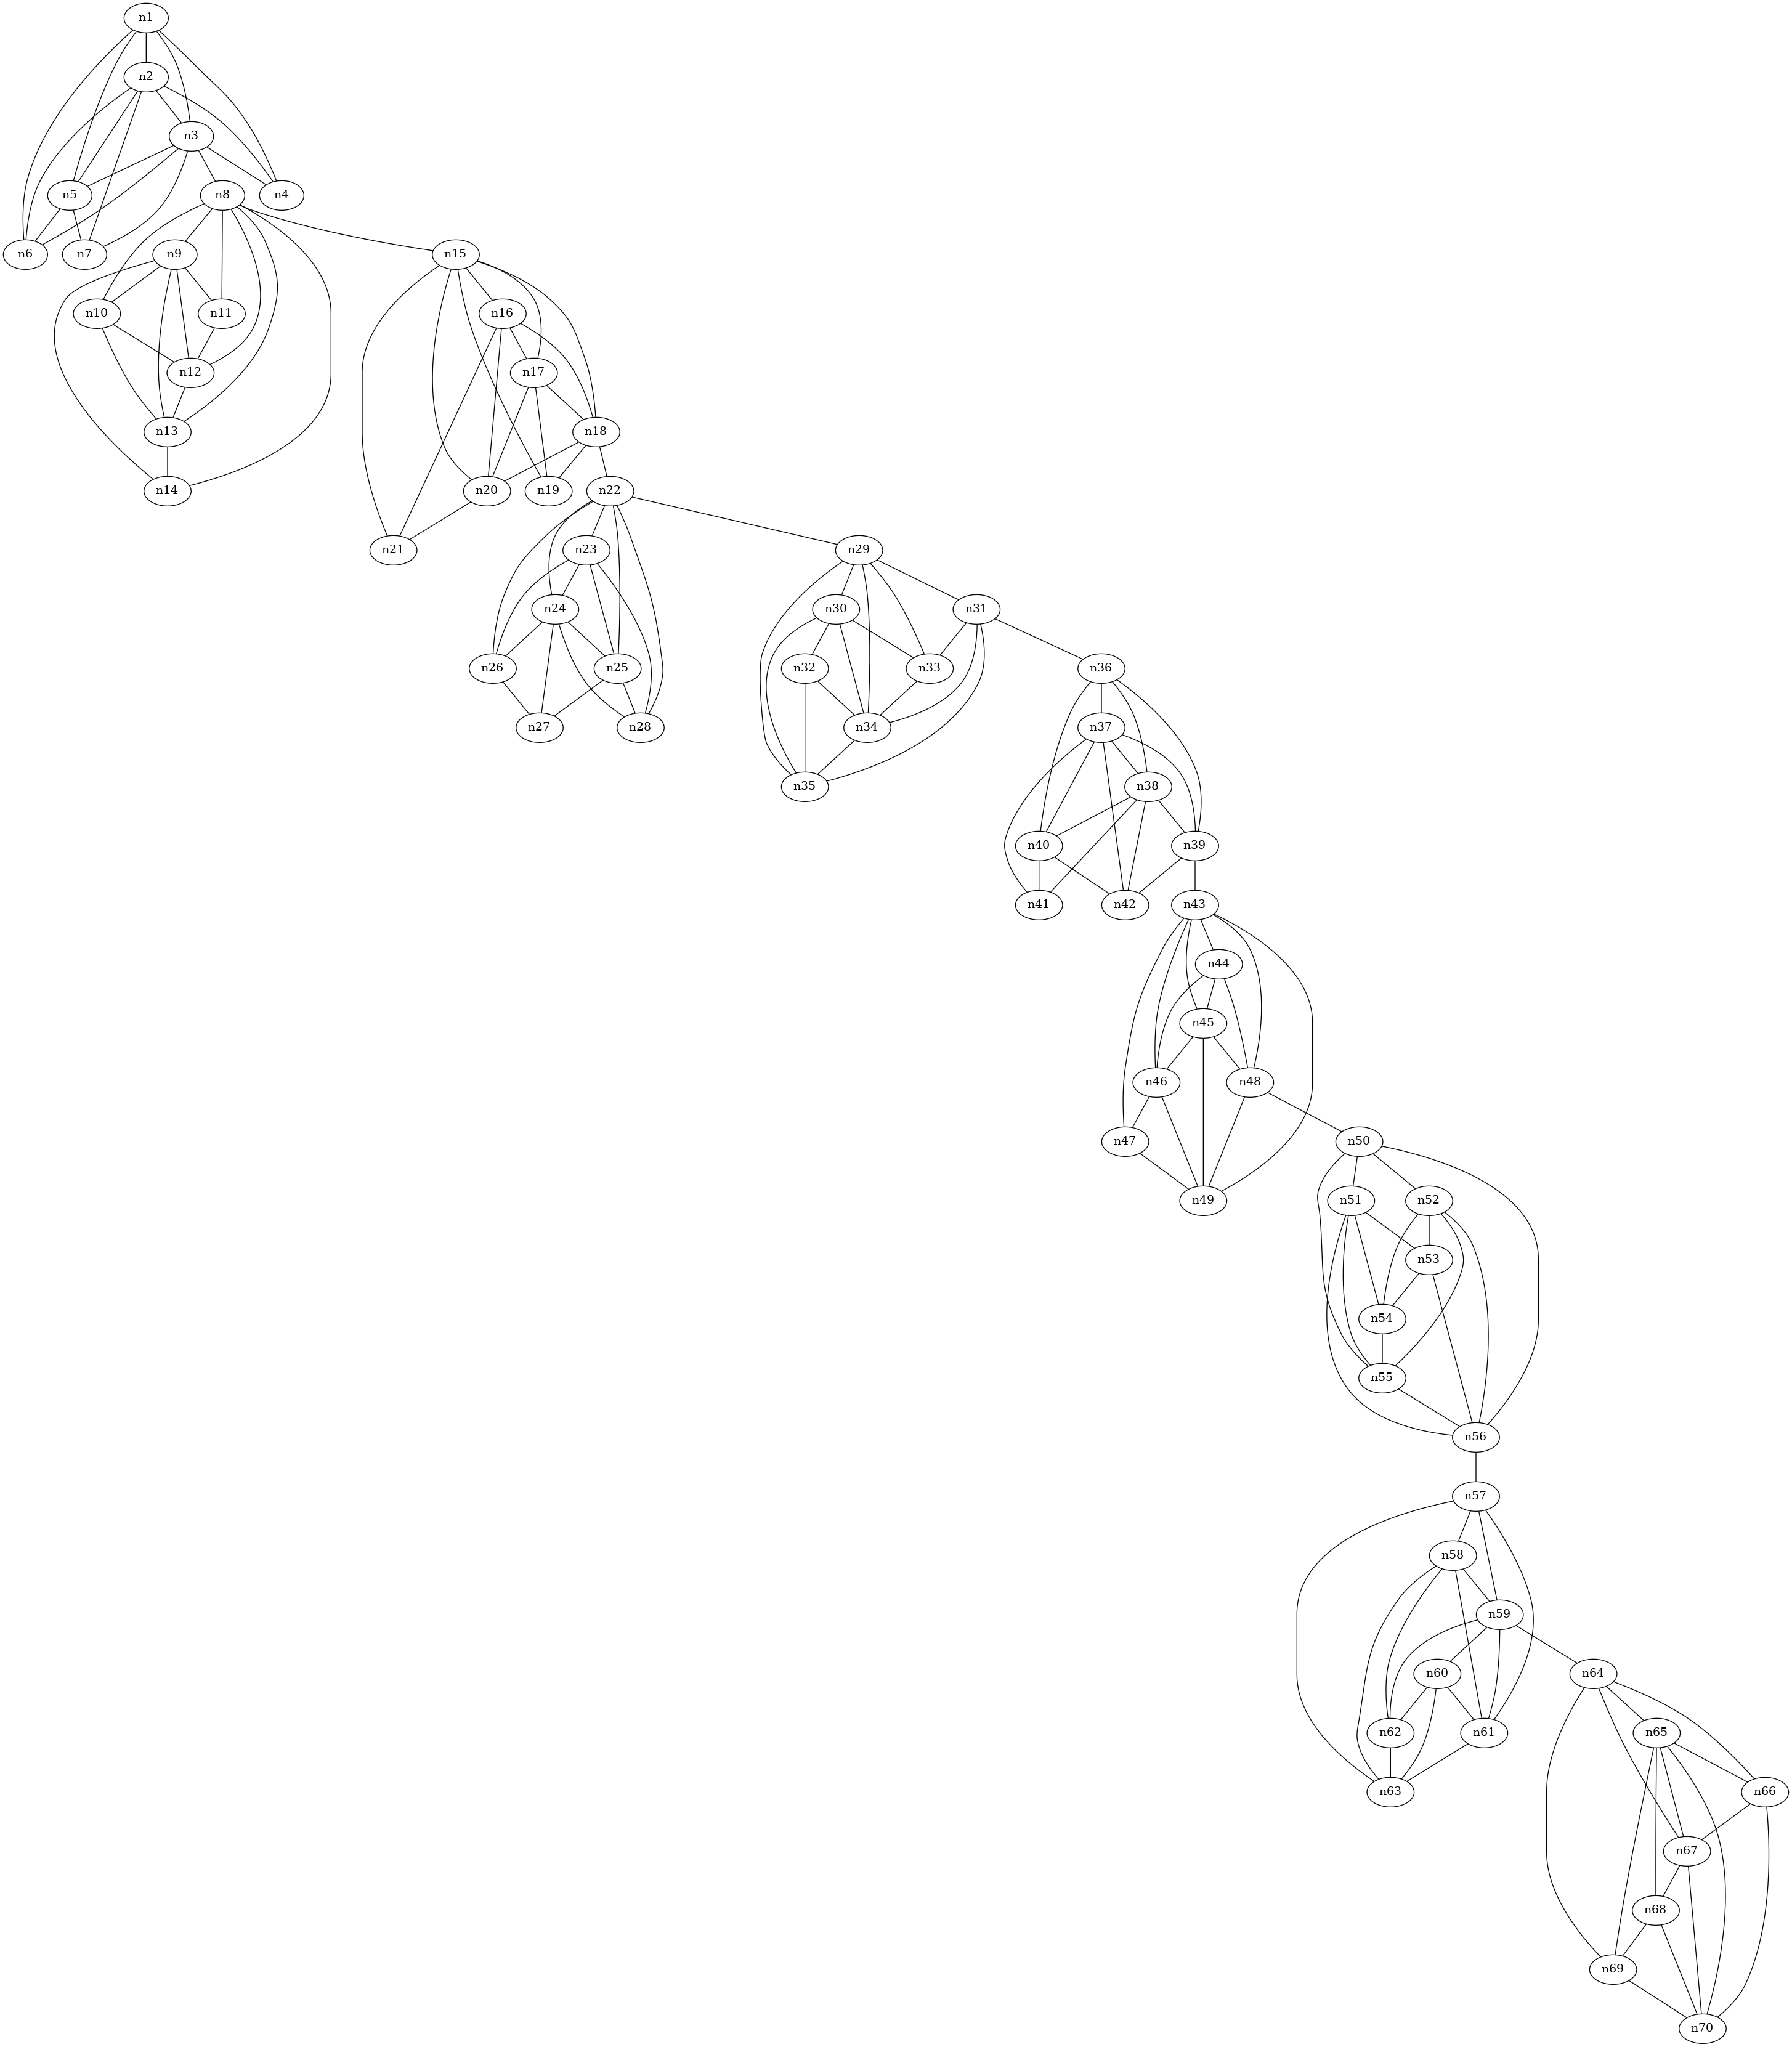
\includegraphics[width=\textwidth]{./ex-inst.png}
\caption{\label{fig:ex-inst}Instance example: special graph structure.}
\end{figure}

This special structure allowed us to design a tailored algorithm exploiting
these 'caves.' The key idea is that as soon as I decide whether I locate a
facility at four connection points adjacent to a cluster, the subproblem
corresponding to this cluster becomes independent of the rest of the problem.
This way I can process clusters one by one and build a BDD encoding the
objective value depending on the choices regarding endpoints only, having width
of at most eight nodes. Such algorithm beats a naive MIP formulation (solved by
Gurobi solver), since it exploits the special structure.

Now, I'd need to add another sort of conditions, to introduce another BDD and
illustrate our BDD-alignment heuristic. First thing I tried was the introduction
of \emph{types} for connection points. That is, I assumed that each one has a type,
and there is a (budget) constraint on the maximum number of points of each type
I can locate a facility at. While the BDD-based approach was indeed faster than
a naive MiP, it was not clear why use our heuristic, since aligning 'type'
diagram to 'cover' diagram to build an intersection later would work just as
well, and in many cases even faster than our simplified-problem-based heuristic.

This is what we had by the previous call. So, we wanted to construct a situation
that would illustrate the practicality of the BDD-alignment heuristic we propose.

\section{t-UFLP + randomized type diagram.}
\label{sec:orgc5dc98a}
Our hypothesis was that we just happened to supply a fortunate initial ordering
by building the type diagram. (So that revising this order to a more complex
cover DD was relatively simple.) Therefore, I tried to destroy this simple
structure to see if it was indeed the case. Viz., before aligning, I randomized
the order of variables in the type diagram. The results in terms of the
resulting intersection diagram sizes are presented in Fig. \ref{fig:intrndpts}.
Here, the red line is just \(y=x\), so a point above the line implies that the
variable-sequence (VS) based heuristic resulted in an intersection diagram with
more nodes than that of the diagram obtained using the simple baseline.

\begin{figure}[htbp]
\centering
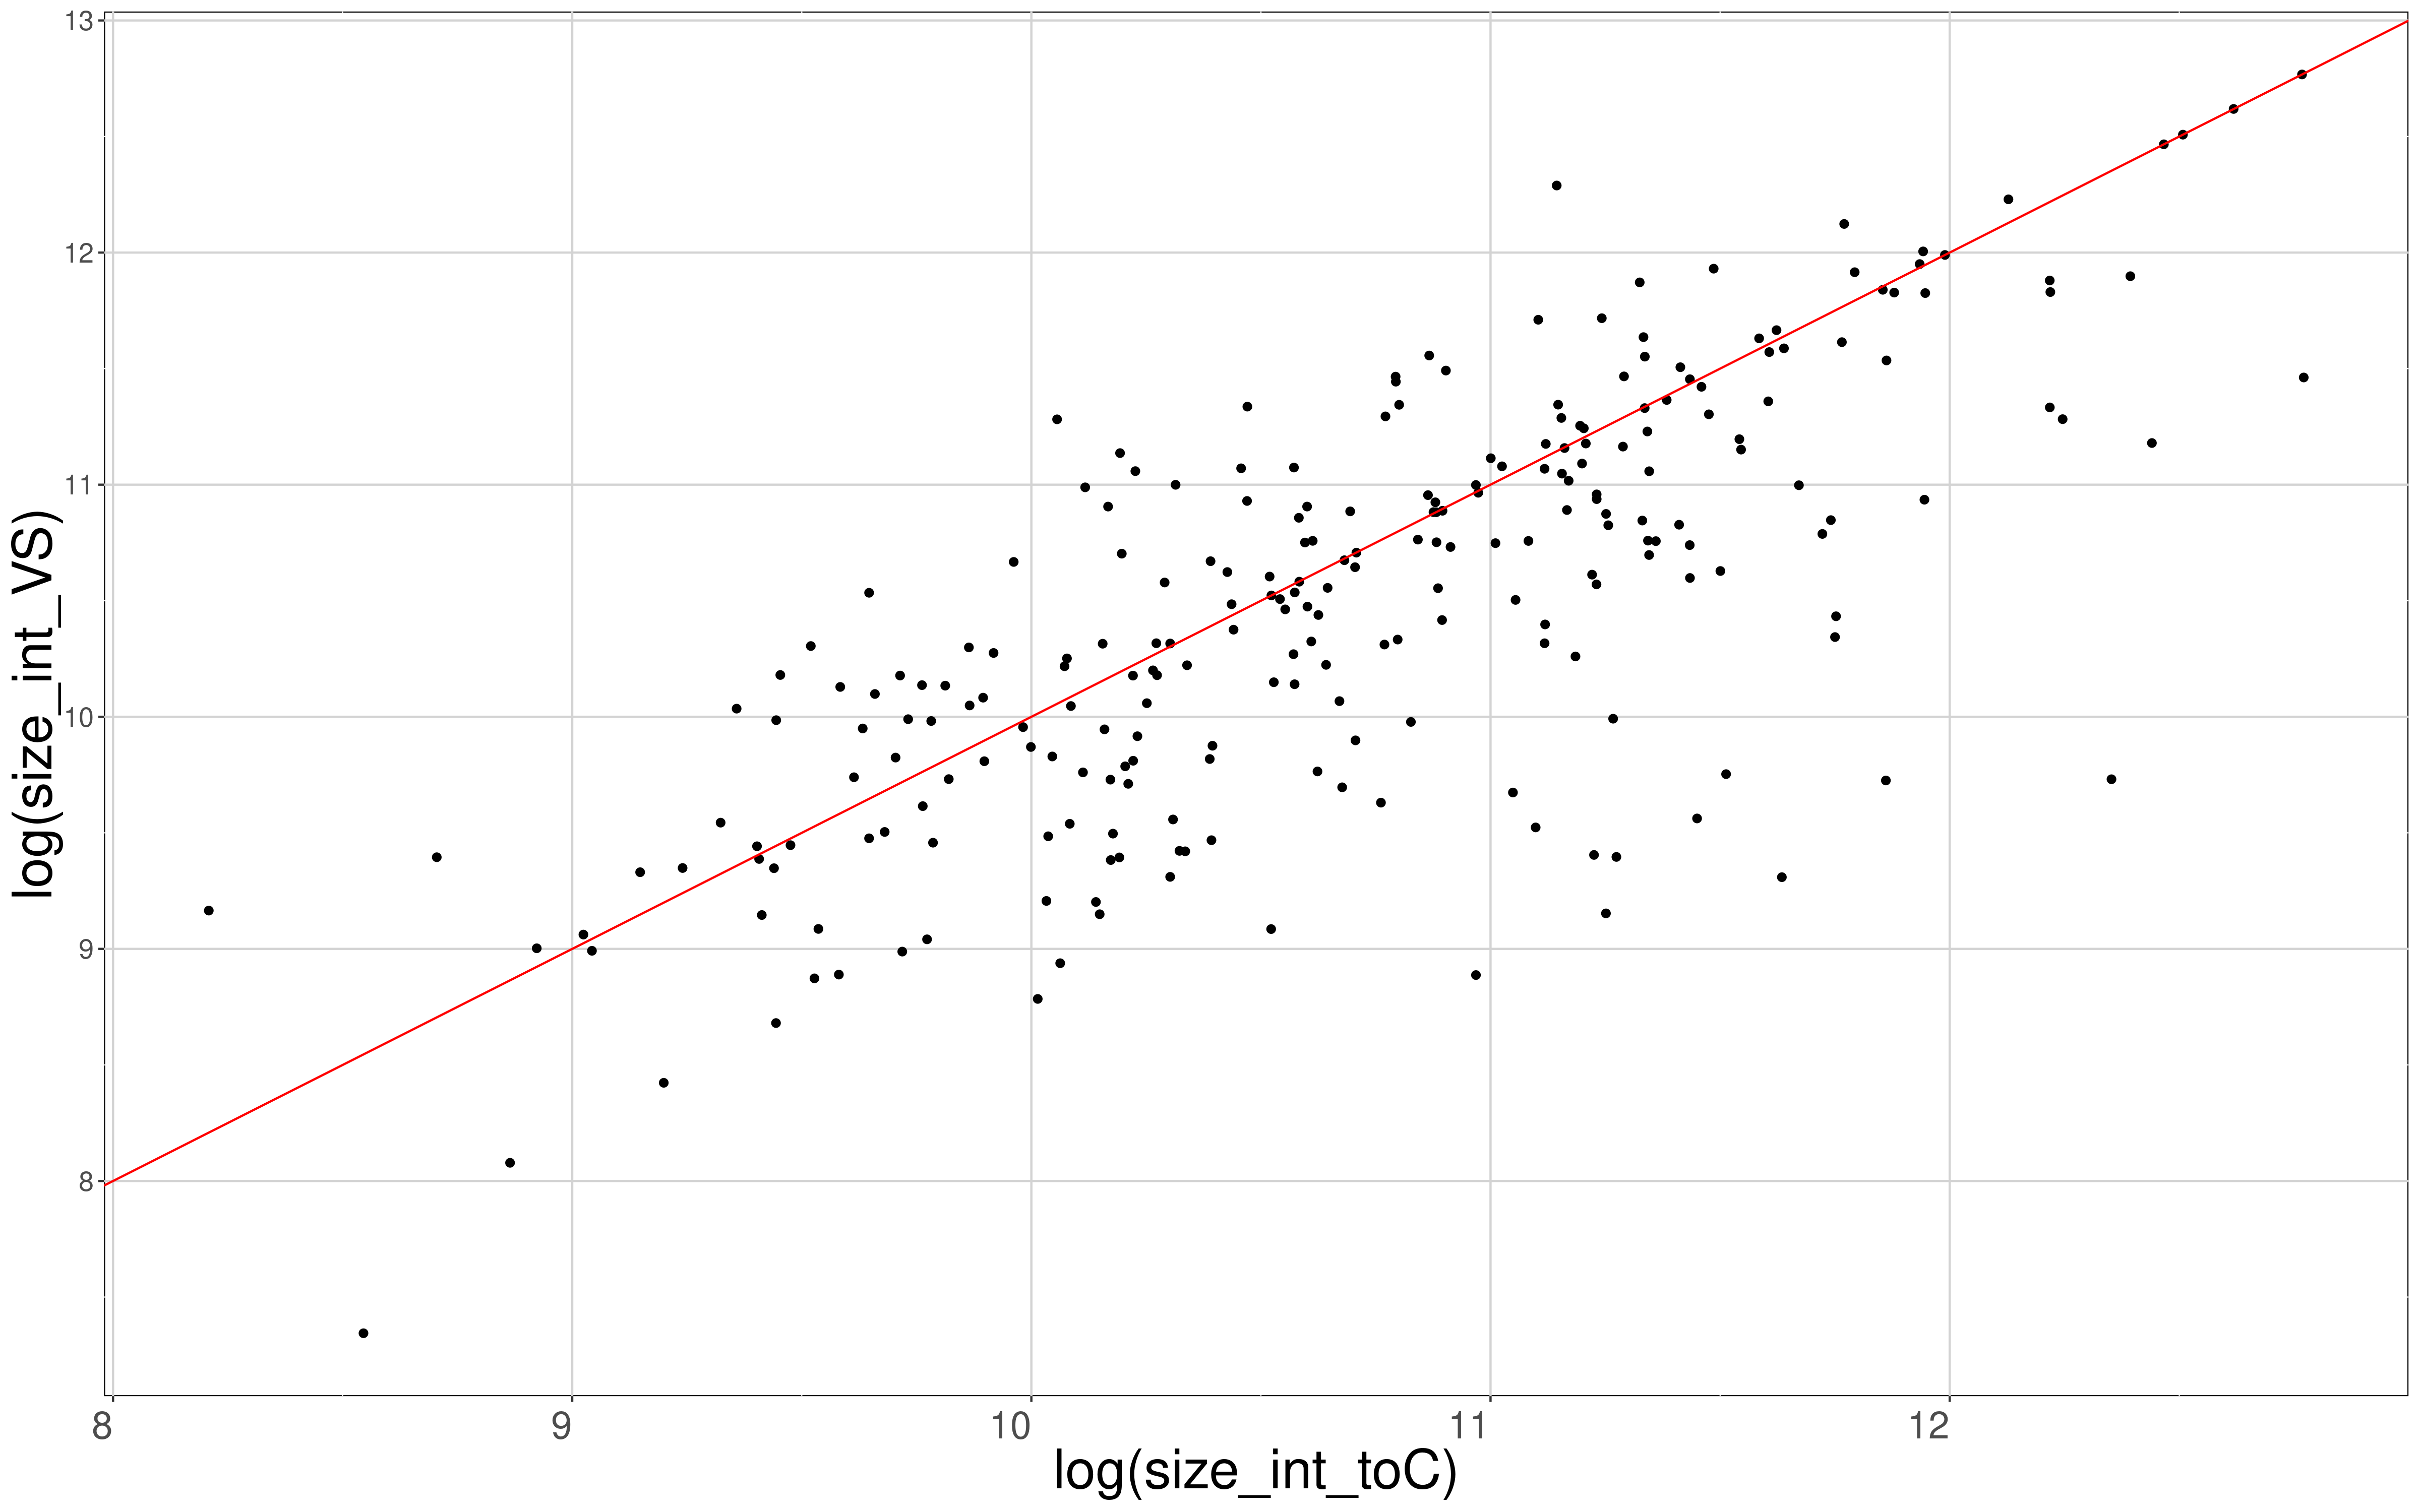
\includegraphics[width=0.8\linewidth]{./int_sizes_points.png}
\caption{\label{fig:intrndpts}Intersection diagram sizes (nominal values), depending on the alignment heuristic used: \texttt{VS} for variable-sequence based, and \texttt{toC} for a simple alternative, "align-to-cover-DD" heuristic.}
\end{figure}

On about 60\% of my random instances (about 62\% if I count the cases when the
size is the same) application of VS-based heuristic yielded smaller intersection
diagrams. This is perhaps more obvious on the histogram of relative intersection
diagram sizes, see Fig. \ref{fig:intrndhist}.

\begin{figure}[htbp]
\centering
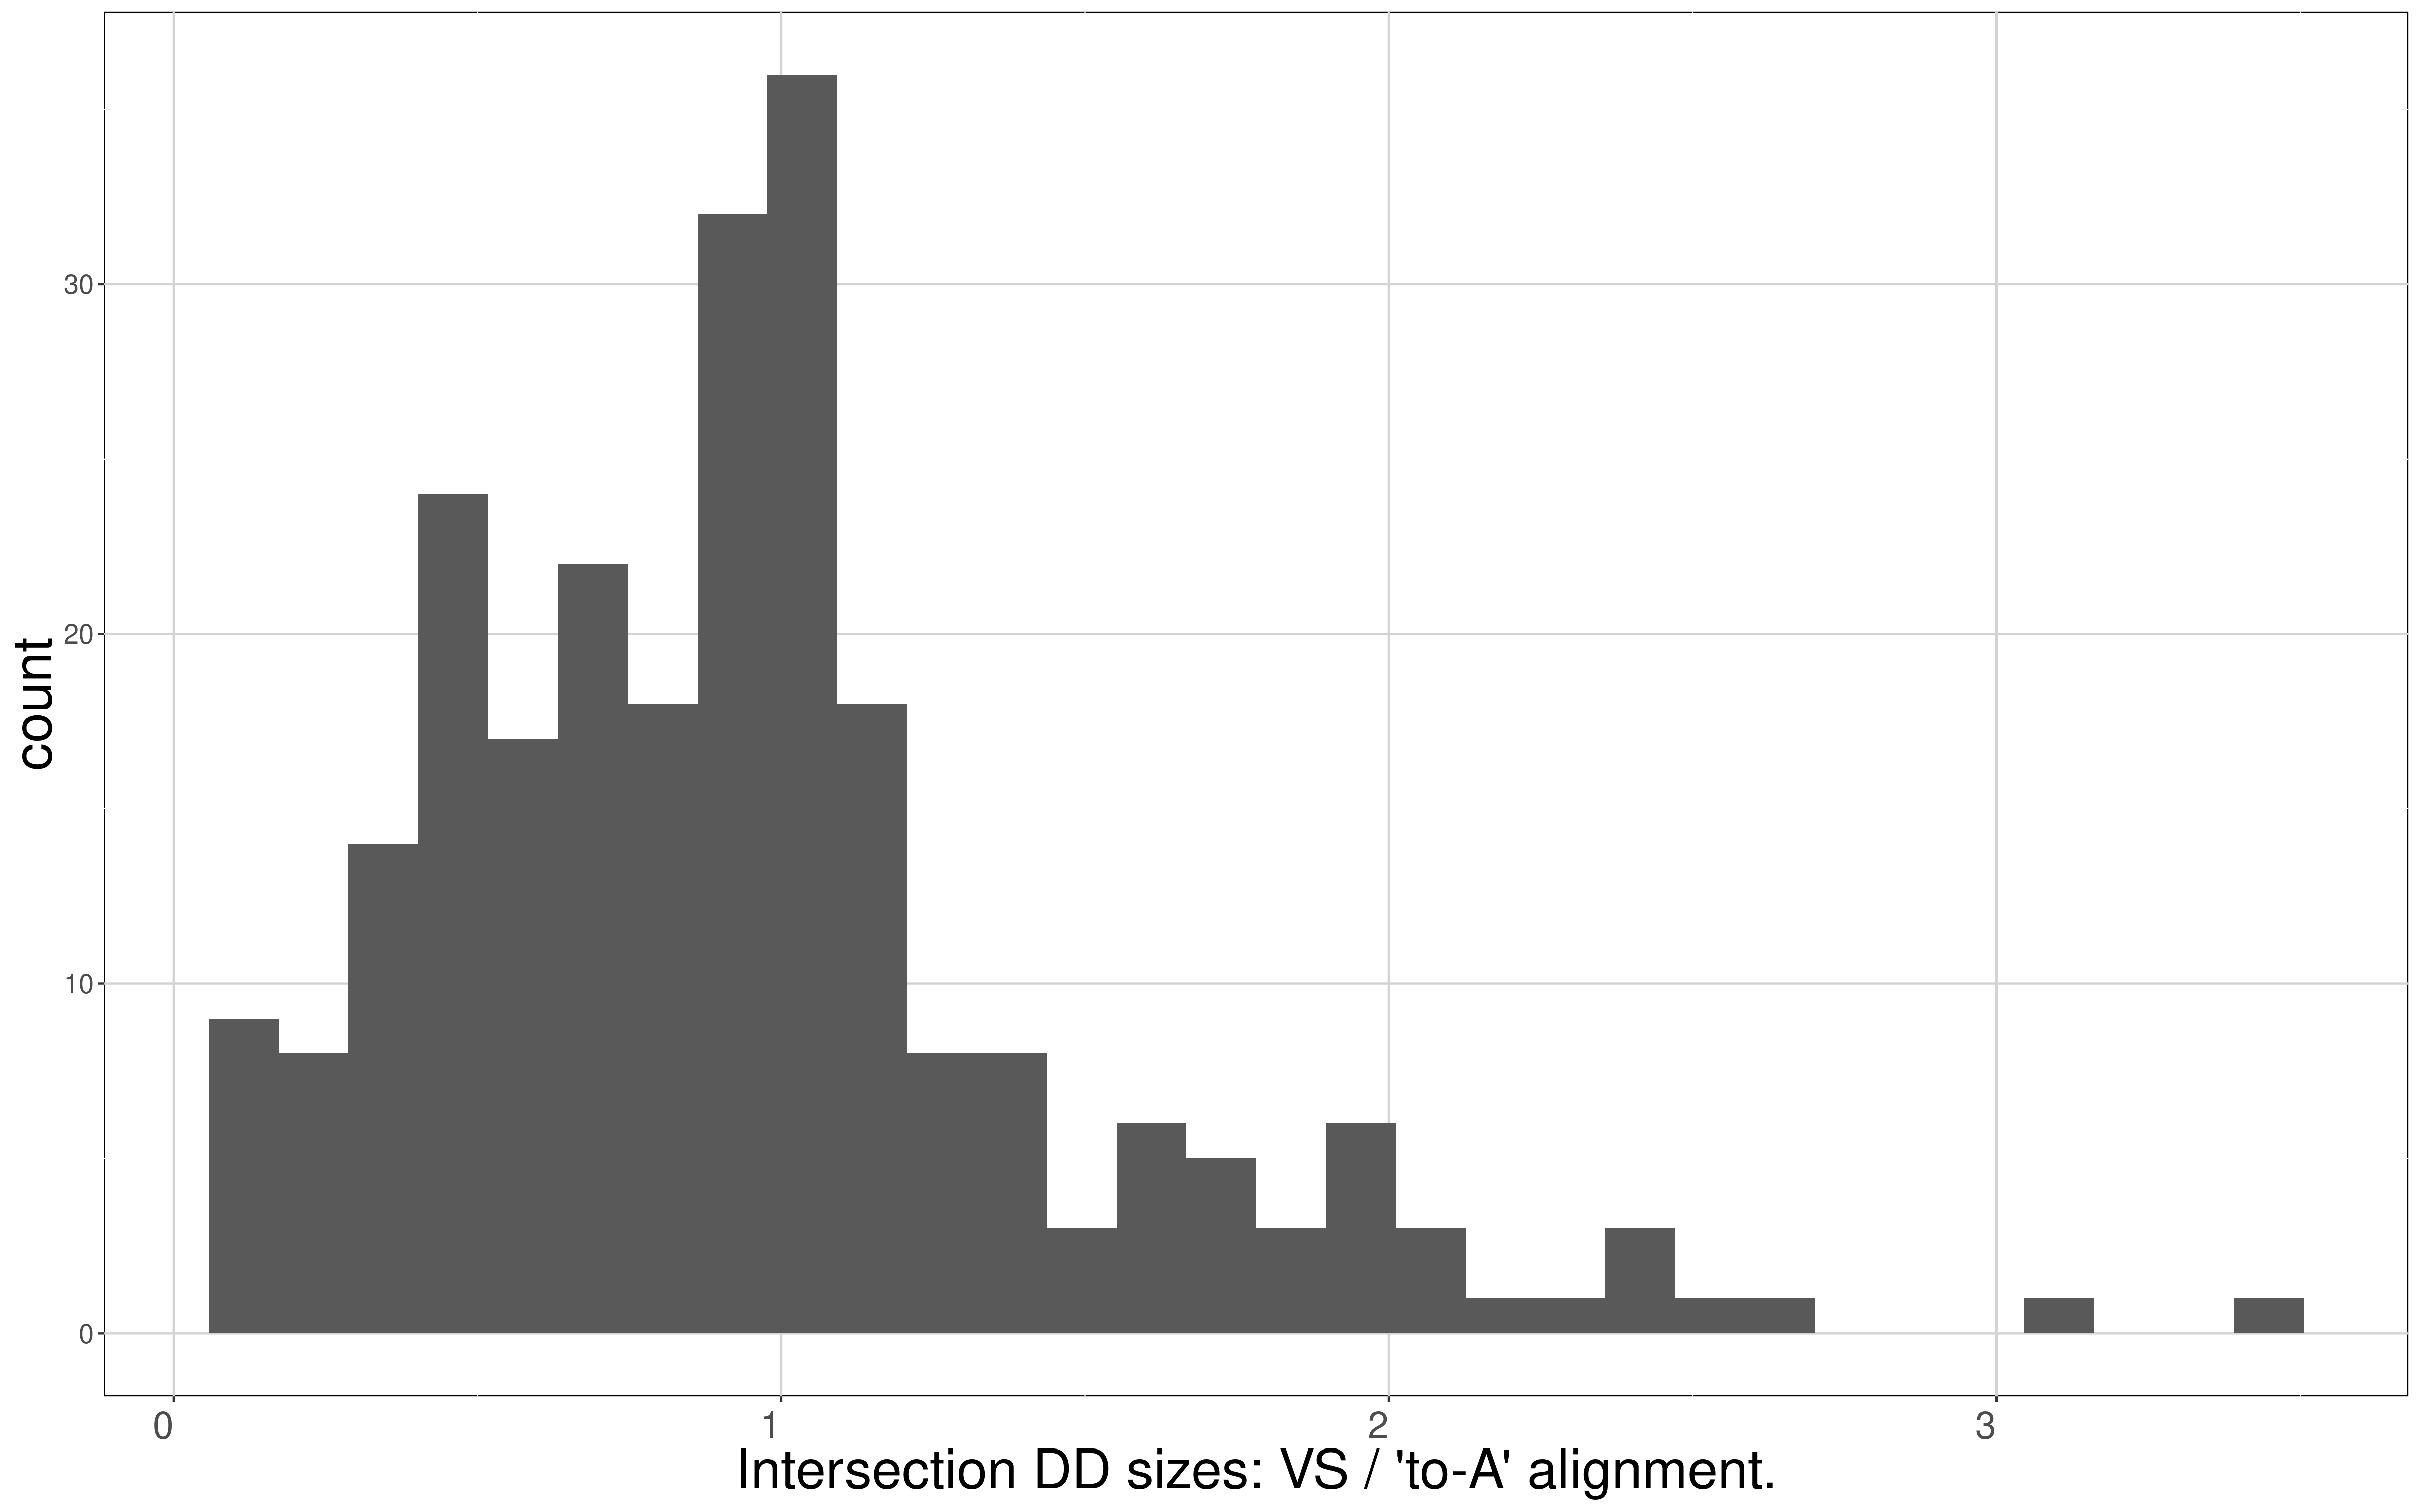
\includegraphics[width=0.8\linewidth]{./int_sizes_hist.png}
\caption{\label{fig:intrndhist}Intersection diagram sizes, VS-based heuristic relative to 'align-to'cover' alternative.}
\end{figure}

Interestingly, runtimes still suggest that the simple baseline heuristic is
comparable, if not faster than the VS-based one; at least with these instances I
have here.

\section{Another variation of `joint-UFLP.'}
\label{sec:org40b5f8e}
Since it seemed that the `type' diagram resulted in some artifacts we'd like to
avoid, I tried to redesign the problem. Again, consider UFLP over this ‘cavemen’
graph with general overlap cost. Let me forget about types altogether, but
assume we have not one, but \textbf{two} such graphs, stitched together via the
connection points in the following sense.

Both graphs possess the special ‘cavemen’ structure, and connection points
coincide. That is, there is a one-to-one mapping between the connection points
in \(G_1\) and the ones in \(G_2\). Moreover, locating a facility at a connection
point in \(G_1\) automatically implies locating the corresponding one in \(G_2\) at
no additional location cost. Otherwise, the two UFLP instances are independent.
I think even the total number of nodes per cluster and for the graph in total
can be different. Overlaps are also calculated for the two graphs independently,
aside from the dependent location decisions.

My primary objective when designing this type of instances was to have a pair of
\textbf{comparable} diagrams to align. I will further try to provide some intuition on
what this problem might actually mean / how to interpret it. However, let’s see
first if it would work for the purposes of the illustration for our heuristic.

I generated random instances as follows:
\begin{enumerate}
\item Create the necessary number of nodes split into the given number of clusters (\(n\) clusters, some fixed number of points each)
\item Make sure that each cluster is connected, and that the clusters are connected to each other as necessary.
\item Create two copies of this graph — these will give me \(G_1\) and \(G_2\).
\item Within each graph, add random edges within each cluster to reach the necessary ‘density’ (parameterized as the number of edges)
\end{enumerate}

The procedure gives me \(G_1\) and \(G_2\), but there is no point in aligning them,
because the sequence of connection points coincide. Therefore, I just rename the
connection points in \(G_2\), by randomizing their order. (I am actually doing
this renaming already after the BDD construction, before the alignment).

In this fashion, I generated 250 random instances and solved them using the
BDD-based approach (naive MIP seems slower anyways), aligning the diagrams using
the variable-sequence-based heuristic (VS) and a simple align-to-A heuristic
(toA). The results are presented in Fig. \ref{fig:jUFLP-hist} --- that's a
histogram of relative intersection diagram sizes, our heuristic relative to the
simple baseline (`align-to-A'). Here, on ca. 90\% of the cases our heuristic performs
better in terms of the sizes. Nominal/absolute runtimes and sizes are depicted
in Fig. \ref{fig:jUFLP-abs}.

\begin{figure}[htbp]
\centering
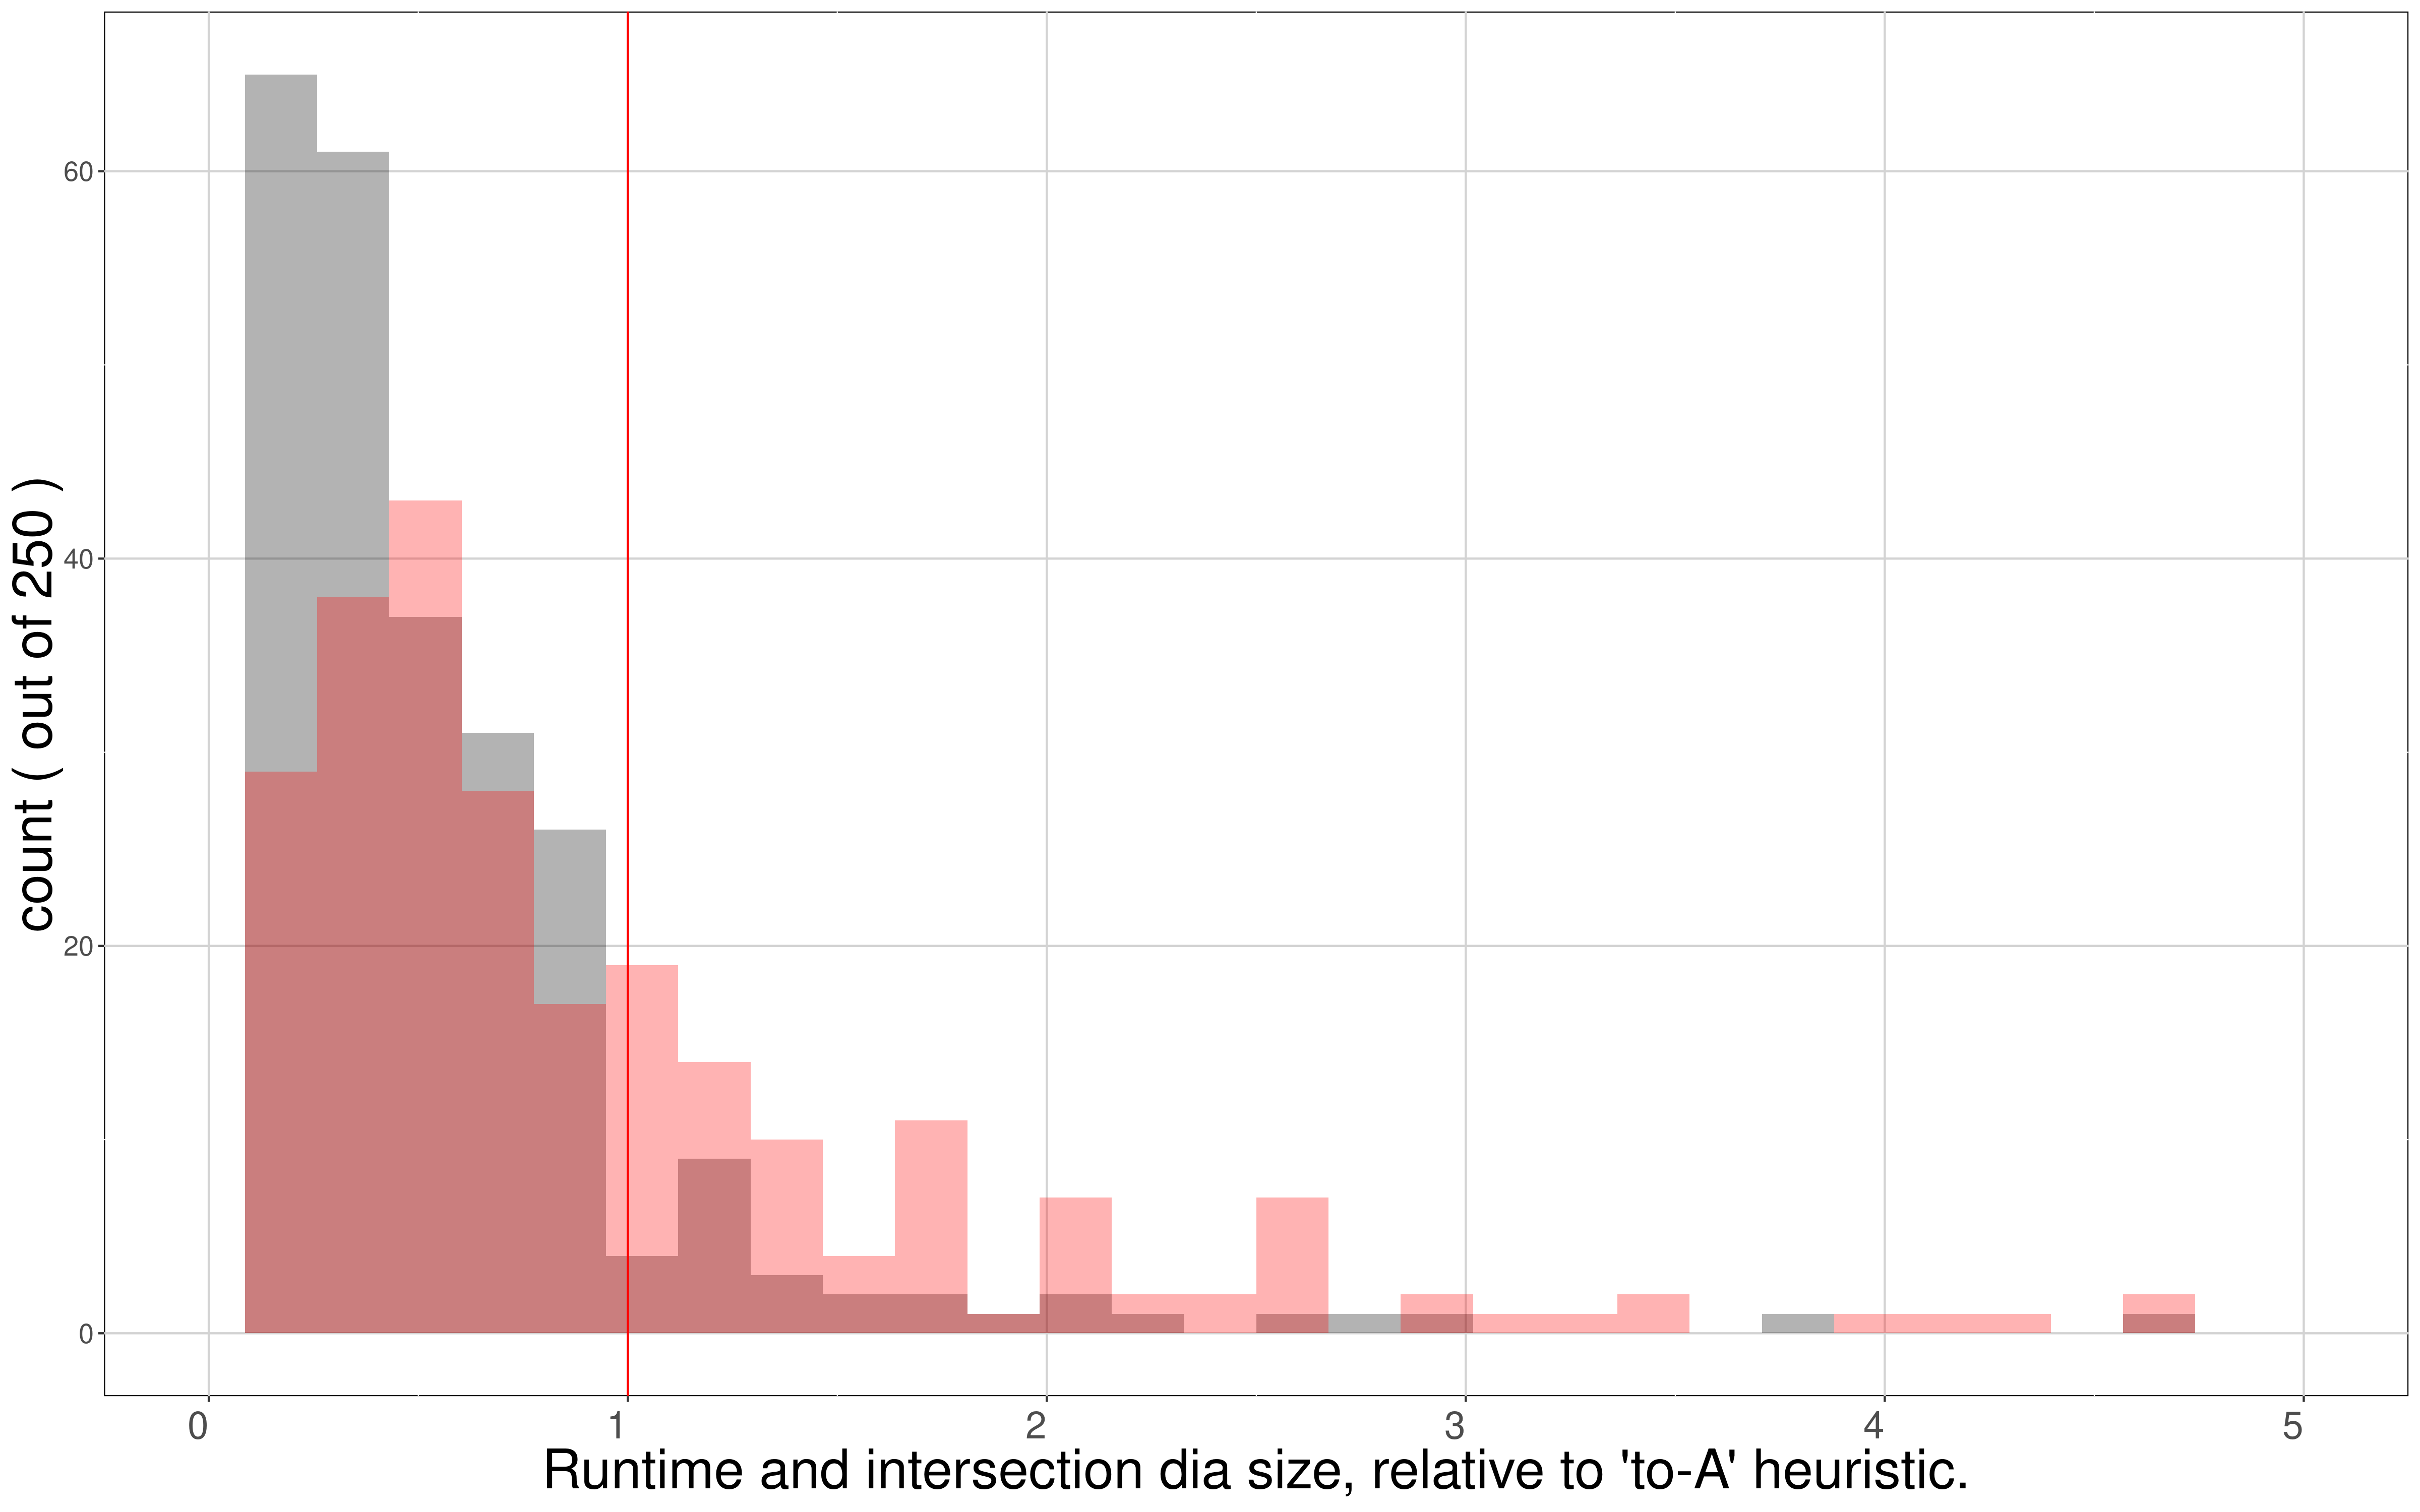
\includegraphics[width=0.9\textwidth]{./jUFLP_hist.png}
\caption{\label{fig:jUFLP-hist}Runtimes for j-UFLP, relative to the simple baseline.}
\end{figure}

  \begin{figure}%
    \centering
    \subfloat[\centering Runtimes, sec.]{{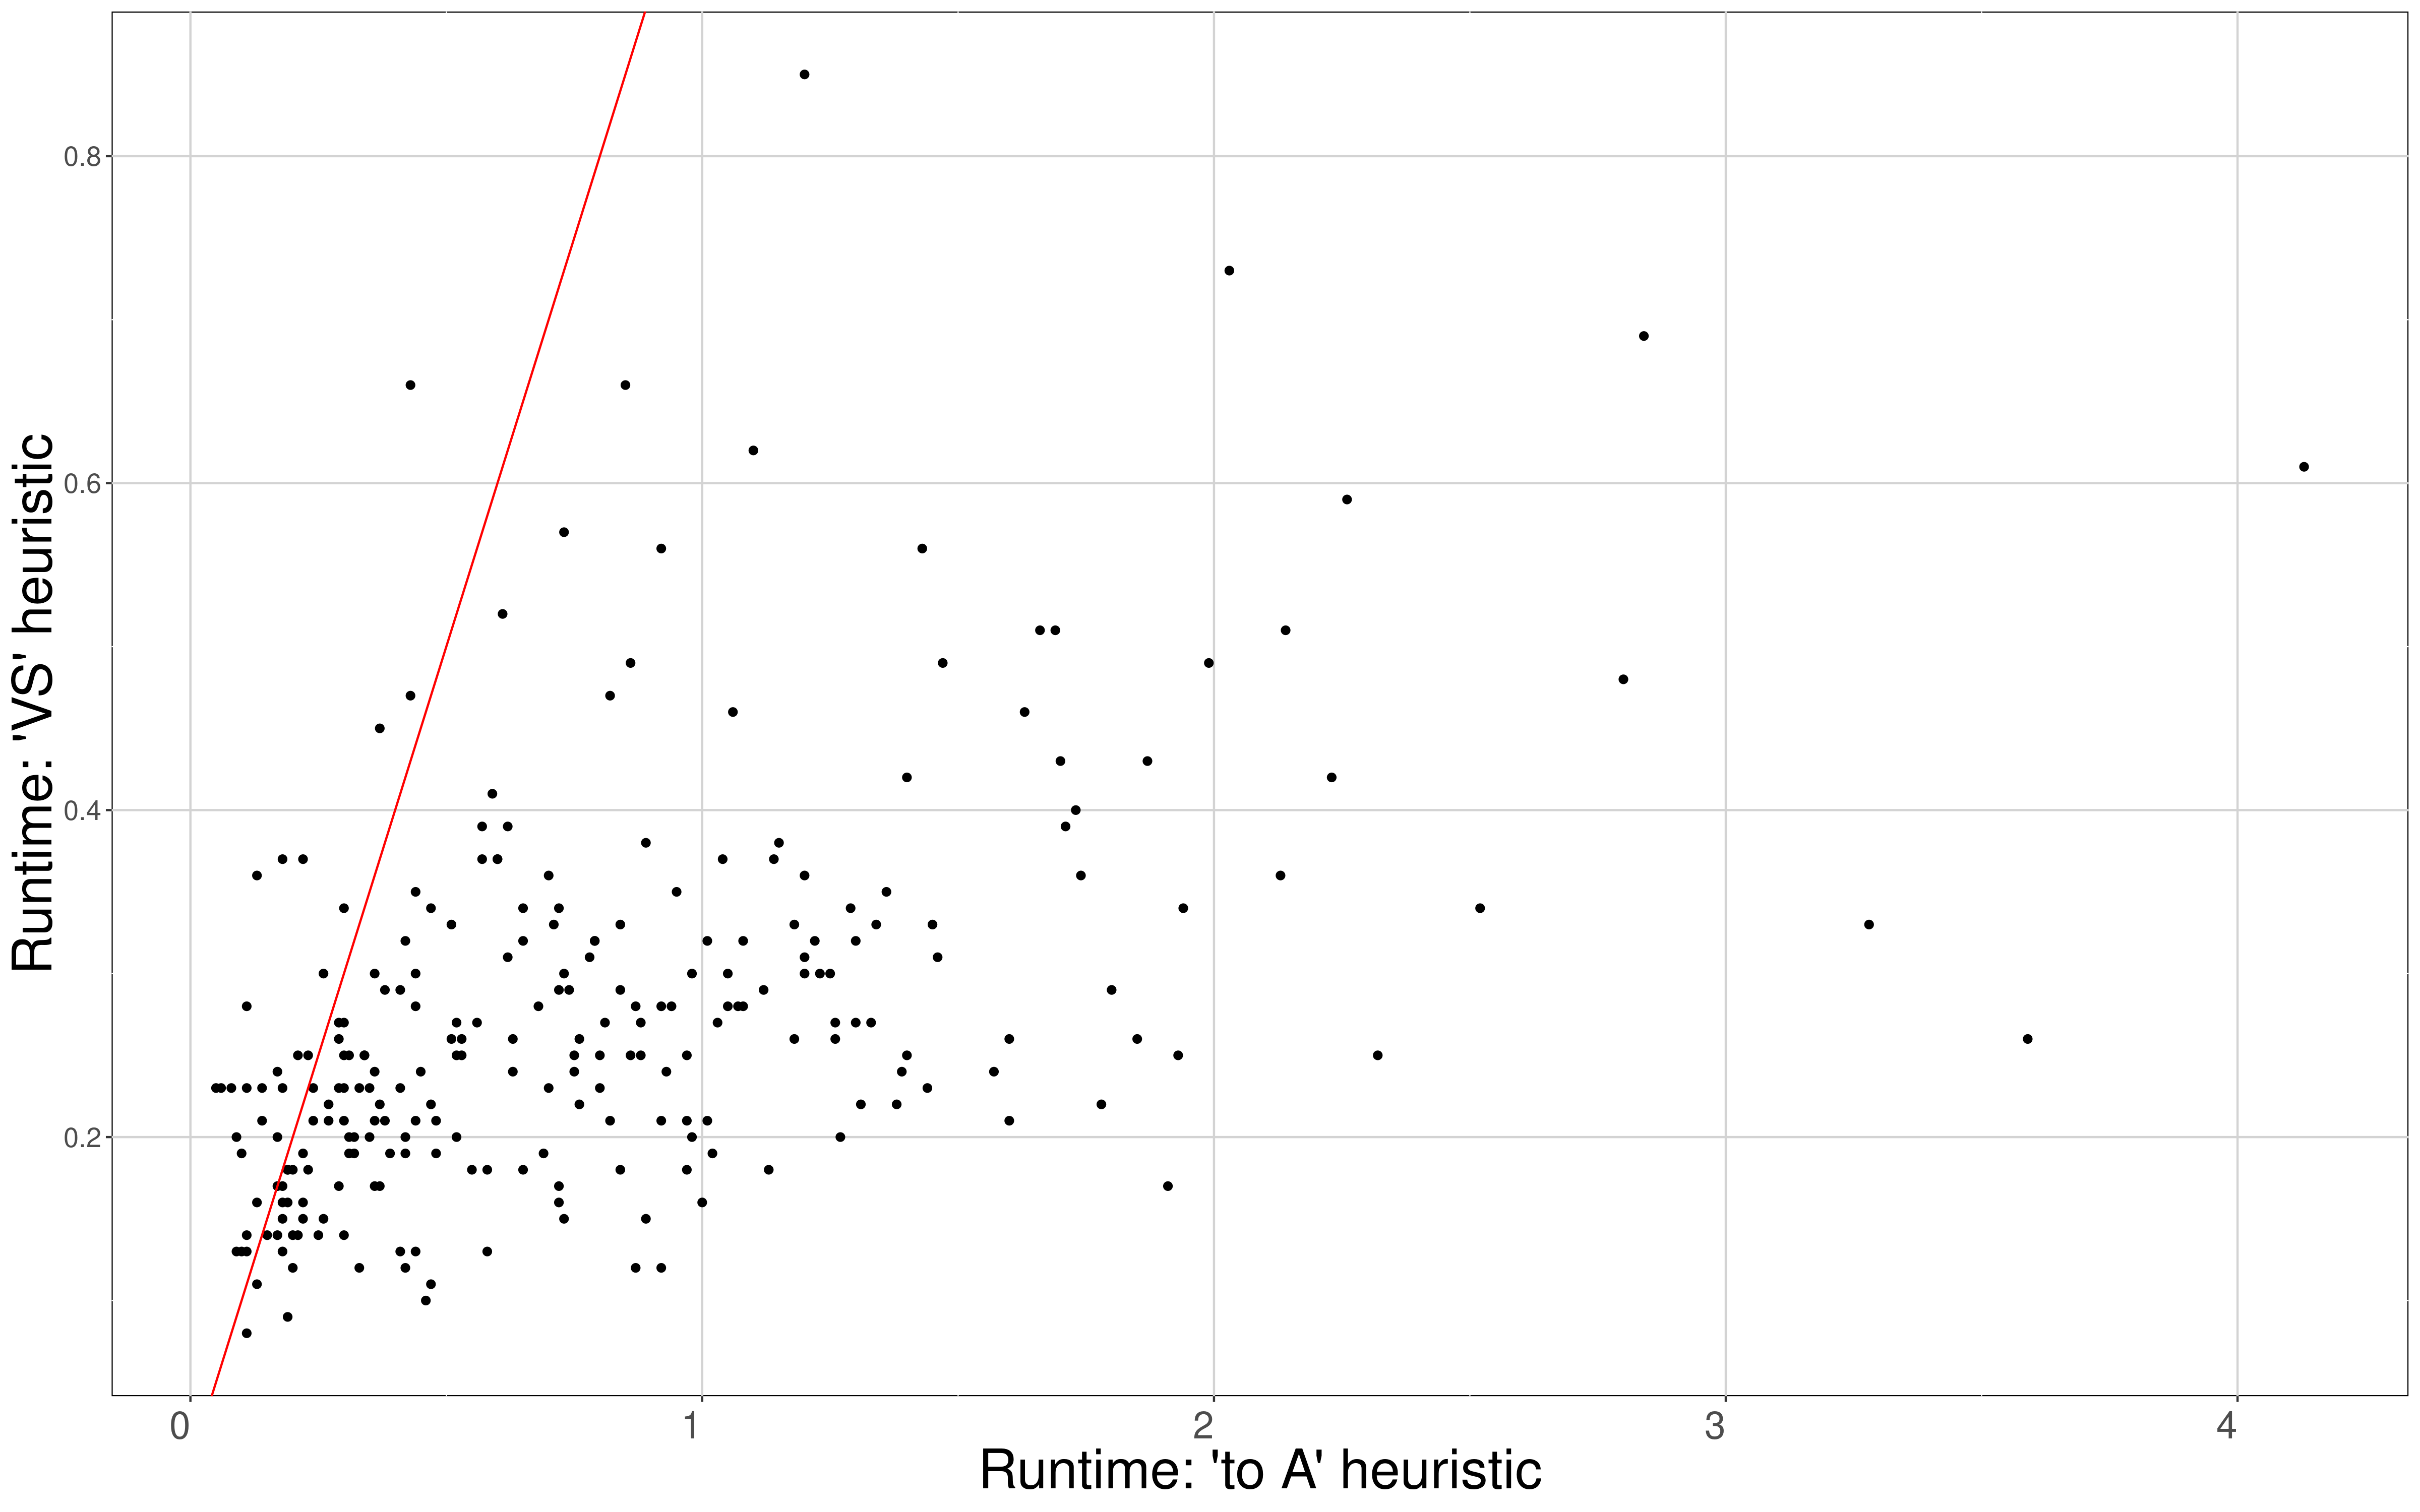
\includegraphics[width=\textwidth]{./jUFLP_runtimes.png} }}%
    \qquad
    \subfloat[\centering Intersection dia sizes, nodes]{{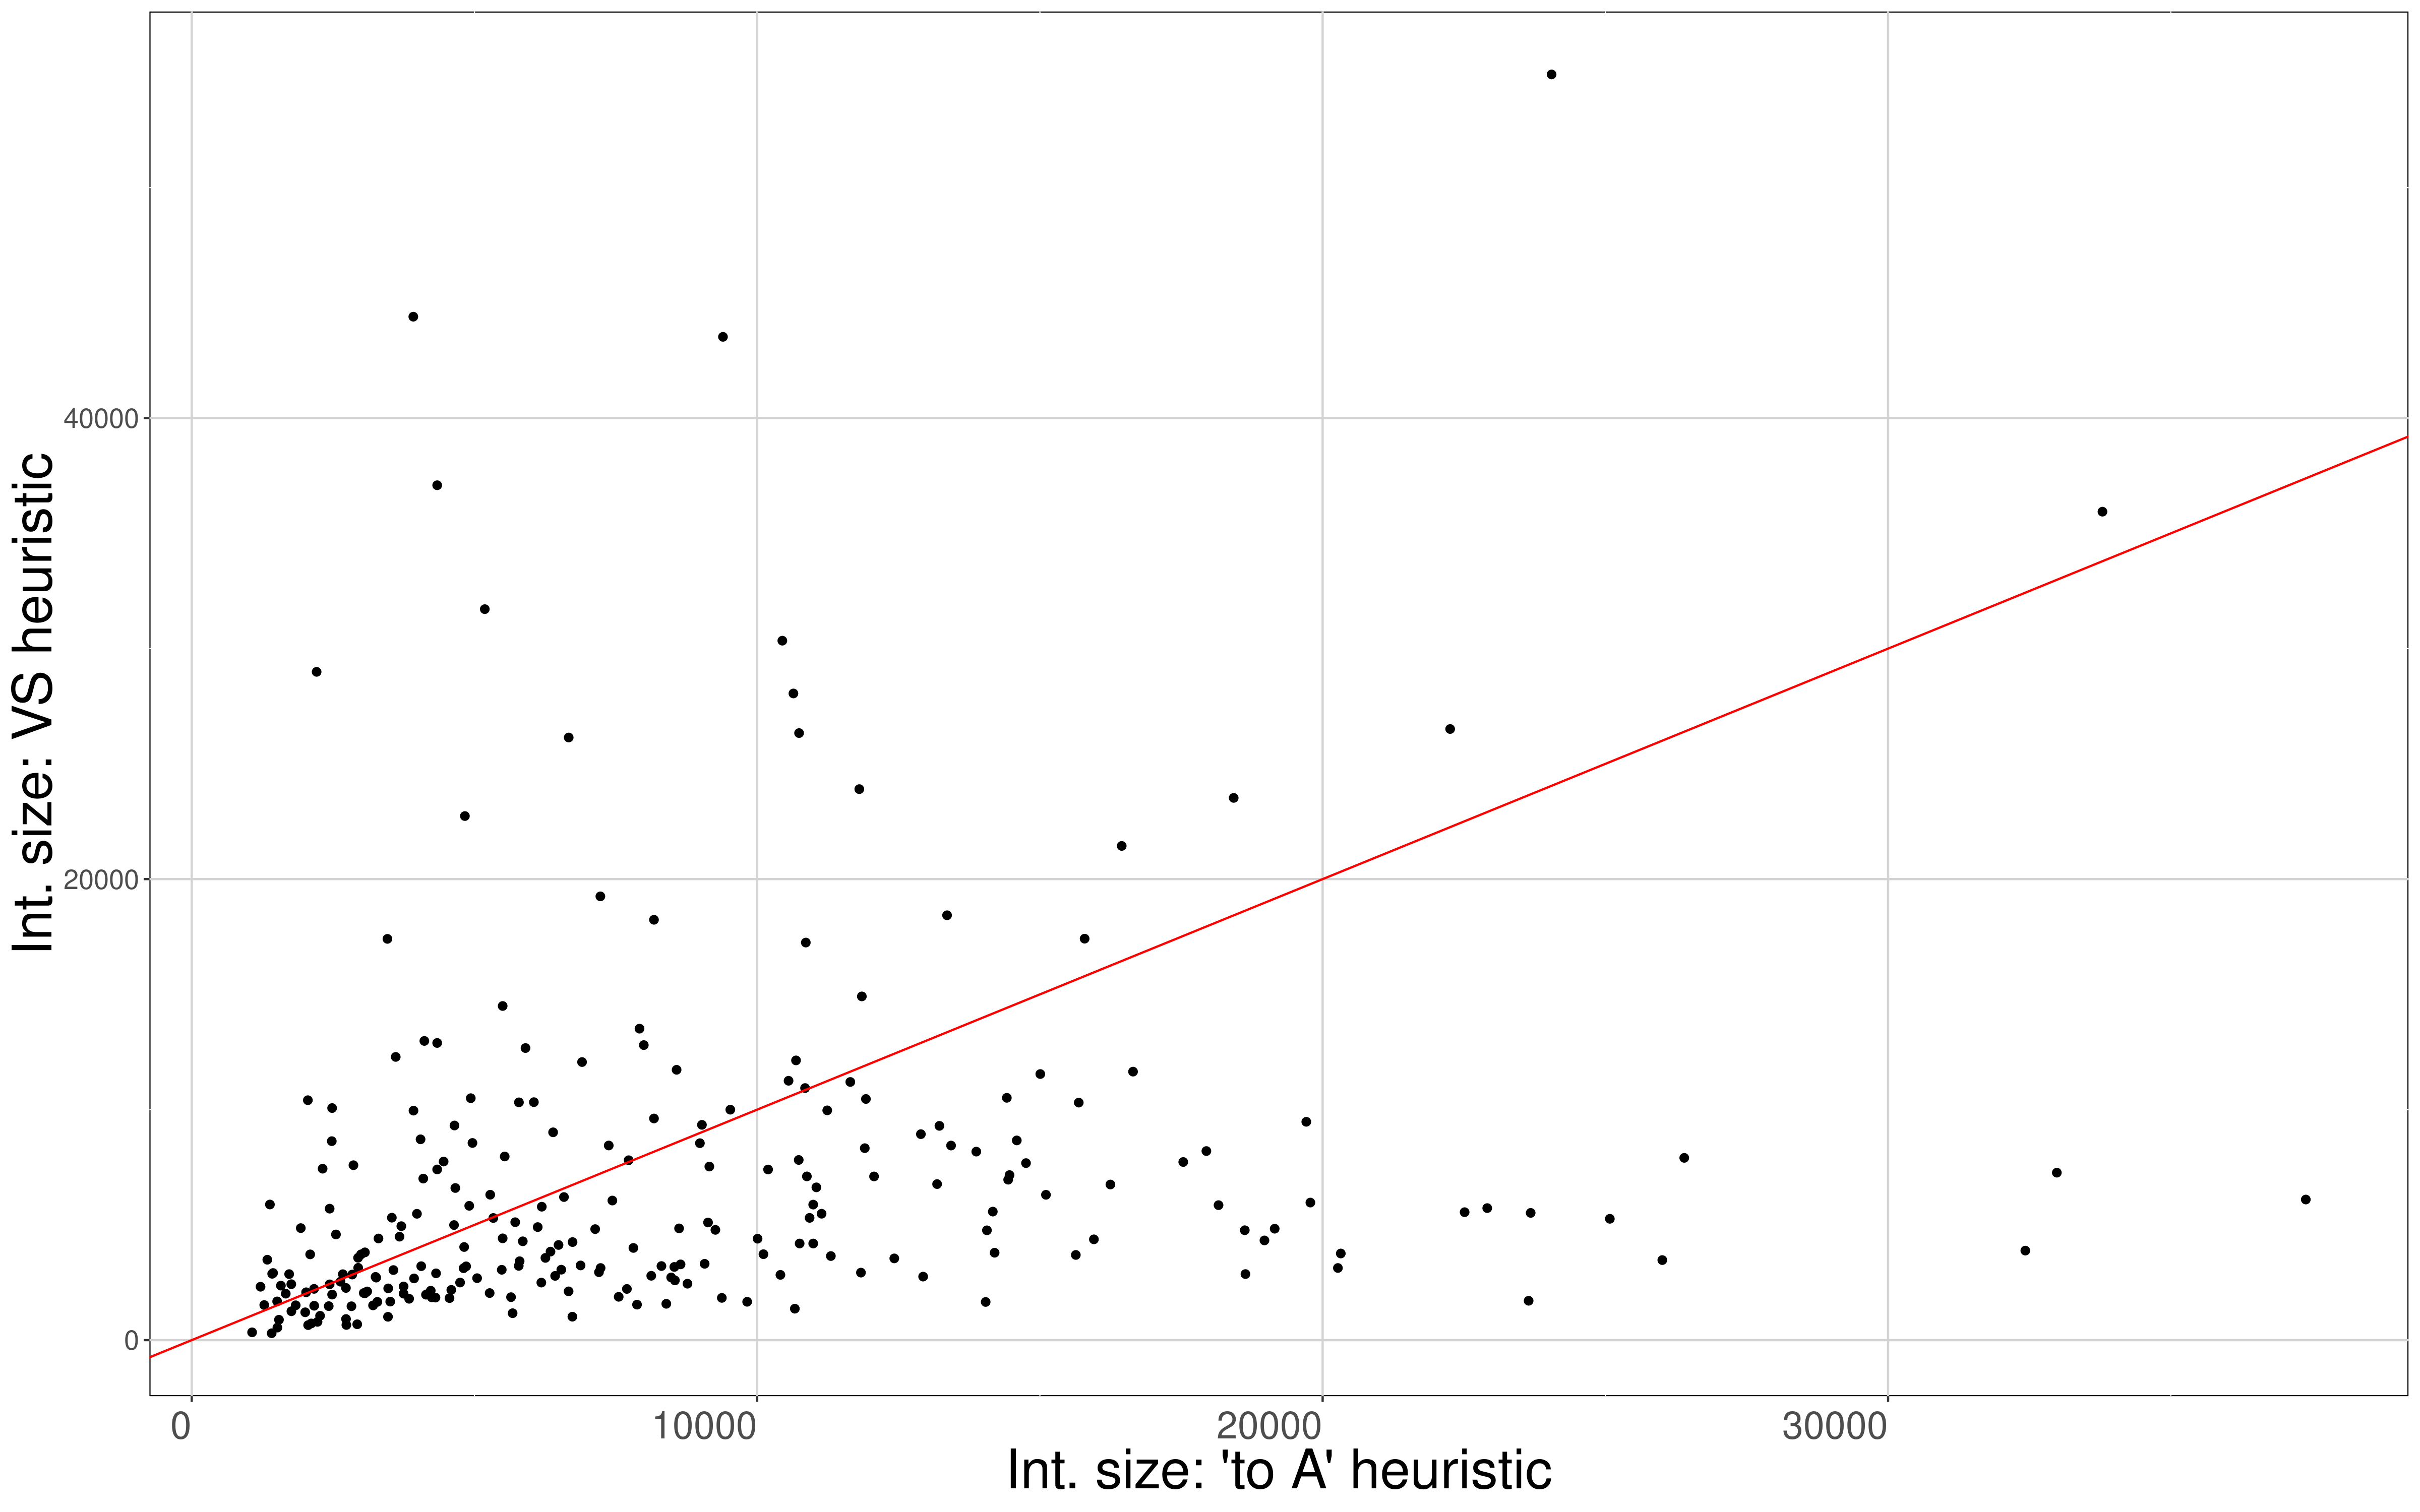
\includegraphics[width=\textwidth]{./jUFLP_sizes.png} }}%
    \caption{Nominal parameters for the two BDD alignment heuristics.}%
    \label{fig:jUFLP-abs}%
\end{figure}

Basically, in this setting it is not obvious how to align the diagrams, and
despite the simple diagram structure, I think the diagrams might explode if we
try to change the variables order carelessly. So, our heuristic beats a naive
one both in terms of runtime and the diagram sizes.

It seems to me this problem would work as an illustration, if we think that it
 is not too theoretical/artificial. Speaking about interpretations, I do not
 have a quite good proposition here. But I would say it is like thinking about
 propagation of information through social graphs of people with respect to
 different interests. For example, my social graph as a researcher is very
 different from my social graph as a hobby Go player. However, I can carry some
 idea or information through both graphs (at least one hop forward), so it makes
 sense that ‘locating’ me just once is enough for both graphs. I do not quite
 see a good intuition why \textbf{connection points} should coincide in the two graphs,
 though. Anyways, I am not sure if it looks solid enough to you, but I would be
 grateful for any hints in this regard!
\end{document}